\section{Структура на проекта}

\begin{figure}[H]
    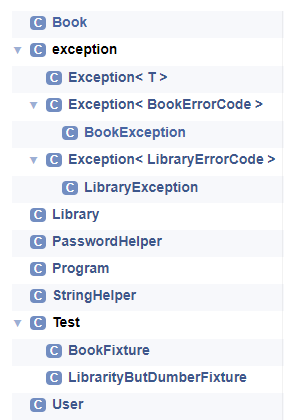
\includegraphics[width=1\textwidth]{project-structure.png}
    \centering
    \caption{Структруа на проекта}
    \label{fig:project-structure}
\end{figure}

Проектът се сътои от три основни компонента:
\begin{itemize}
    \item Книга (Book), която има име, автор, описание, име, автор, описание, рейтинг, международен стандартен номер (ISBN), както и съдържание, което е записано в текстов файл. Книгата предоставя достъп до полетата си и до съдържанието си.

    \item Потребител (User), който има потребителско име, потребителска парола и информация за това дали има администраторски права. Потребителя предоставя достъп до потребителското си име и до това дали е администратор, но не и до паролата си. За да се потвърдят набор от потребителски данни, е предоставен метод за вход.

    \item Библиотека (Library), която оправлява списък с потребители и списък с книги. Борави и с двоични файлове, където записва съдържанието на списъците, когато това се изисква. Има механизми за вход на потребители и смяната на тяхната парола. Също така има механизми за менежиране на списъка с книги.
\end{itemize}